\documentclass[preprint]{sigplanconf}

\usepackage{amsmath}
\usepackage{amssymb}
\usepackage{stmaryrd}
\usepackage[pdftex]{graphicx}

\begin{document}

\newcommand{\etrans}[1]{\mathcal{E} \llbracket #1 \rrbracket}
\newcommand{\dtrans}[1]{\mathcal{D} \llbracket #1 \rrbracket}
\newcommand{\ttrans}[1]{\mathcal{T} \llbracket #1 \rrbracket}
\newcommand{\strans}[1]{\mathcal{S} \llbracket #1 \rrbracket}
\newcommand{\trans}[1]{\llbracket #1 \rrbracket}

\newcommand{\tot}{\leftrightarrow}

\newcommand{\unr}{\texttt{UNR}}
\newcommand{\bad}{\texttt{BAD}}
\newcommand{\any}{\texttt{Any}}
\newcommand{\ok}{\texttt{Ok}}
\newcommand{\hprime}{\mathcal{H}'}
\newcommand{\cfc}{\texttt{CF}}
\newcommand{\cf}[1]{\texttt{CF}(#1)}
\newcommand{\weak}[1]{\mbox{$\$$weak}(#1)}
\renewcommand{\min}[1]{\mbox{$\$$min}(#1)}


\title{Static contract checking for Haskell}
\maketitle

\section{Introduction}

Our approach to static contract-checking is to translate source code
to a first-order logic theory and then use an automated theorem prover
to check the consistency of the theory.

Consider:
\begin{verbatim}
data List a = Nil | Cons a (List a)

notnull x = case x of
  Nil -> False
  Cons(x,y) -> True

head ::: (CF && {x | notnull x }) -> CF
head xs = case xs of
  Nil -> BAD
  Cons(x,y) -> x
\end{verbatim}

First, we need to encode the List structure. 

We start by stating that $Nil$ and $Cons$ can never be equal:
\begin{equation*}
\forall a,b.~Cons(a,b) \neq Nil
\end{equation*}

Then, we must state that $Nil$ never crashes (ie cannot be evaluated
to an exception) and that $Cons(x,y)$ crashes iff either $x$ or $y$
crashes. The statement $x$ crashes is encoded by the term $\cf{x}$.

\begin{equation*}
\cf{Nil}
\end{equation*}
\begin{equation}
  \label{cfcons}
\forall a,b.~\cf{a} \land \cf{b} \iff \cf{Cons(a,b)}
\end{equation}

We also say some stuff about unreachibility but I can't think of a
good way to explain it right now.
\begin{equation*}
\forall y,ys.~Cons(y,ys) \neq \unr 
\end{equation*}
\begin{equation*}
Nil \neq \unr 
\end{equation*}

Finally, we define projections for $Cons$. It is not strictly
necessary, but it will be handy:
\begin{equation**}
\forall xs,y,ys.~sel_{1,Cons}(Cons(y,ys)) = xs \implies xs = y 
\end{equation**}
\begin{equation*}
\forall xs,y,ys.~sel_{2,Cons}(Cons(y,ys)) = xs \implies xs = ys 
\end{equation*}

Now we translate the $null$ function. Note that the symbols $true$ and
$false$ are the representation of the data constructors $True$ and
$False$ in Haskell, not the boolean values $\top$ and $\bot$ in our
logic.
\begin{equation*}
\forall xs.~ xs=Nil \implies notnull(xs) = false
\end{equation*}

\begin{equation}
  \label{defnotnull}
\forall xs,y,ys.~ x=Cons(y,ys) \implies notnull(xs) = true
\end{equation}

We also need to specify the translation of calls to $notnull$ with
$\bad$ values (to encode the fact that $notnull(\bad) = \bad$.
\begin{equation*}
\forall xs.~xs=\bad \to notnull(xs) = \bad
\end{equation*}

Finally, we say that one call $notnull$ with a an argument which is
not $Nil$ or $Cons$ or $\bad$ then the result is $\unr$.
\begin{align}
  \label{unrnotnull}
  \forall xs.~xs \neq \bad \land xs \neq Nil  \notag \\
  \land xs \neq Cons(sel_{1,Cons}(xs),sel_{2,Cons}(xs)) \to  \notag \\
  notnull(X) = \unr 
\end{align}

The translation of $head$ follows the same pattern:
\begin{align}
  \forall xs.~ x=Nil \implies head(xs) = \bad \notag\\
  \forall xs,y,ys.~ x=Cons(y,ys) \implies head(xs) = y     \label{defhead} \\
    \forall xs.~xs=\bad \to head(xs) = \bad \notag
\end{align}

\begin{align*}
 \forall xs.~xs \neq \bad \land xs \neq Nil \notag \\
 \land xs \neq Cons(sel_{1,Cons}(xs),sel_{2,Cons}(xs)) \to  \notag \\
 head(X) = \unr 
\end{algin*}

We now have translated the source code. Let us call all those formulae
the theory $T$. We translate separatly the contract:
\begin{equation*}
  \phi := \forall xs.~\cf{xs} \land notnull(xs) = true \to \cf{head(xs)} 
\end{equation*}

Now that we translated everything to first-order logic, we can ask the
theorem prover if the theory formed by those formulae is
consistent, ie if $T \vdash \phi$.

Intuitively, $T$ is consistent (ie $T \not \vdash \bot$), because each
formula serves a specific purpose. Now, assume that $xs$ satisfies
$\cf{xs}$ and $notnull(xs) = true$.  We can derive that $xs \neq \bad$
because we have $\cf{xs}$ and $\lnot \cf{\bad}$. The constraint
$notnull(xs) = true$ doesn't directly imply that $xs = Cons(y,ys)$ for
some $y$ and $ys$. But $notnull$ is totally defined, because of
\eqref{unrnotnull}. This implies (by \eqref{defnotnull}) that there exist
$y$ and $ys$ such that $xs = Cons(y,ys)$. Recalling $\cf{xs}$, we can
now derive $\cf{y}$ and $\cf{ys}$ (by \eqref{cfcons}). But $head(xs) =
y$ because of \eqref{defhead}, and $y$ is crash-free, so we can finally
derive $\cf{head(xs)}$. QED.


\section{Languages}
\subsection{$\hprime:~\lambda$-calculus variant}

The syntax of $\mathcal{H}$ is defined in \ref{hprime-stx}. A module
is a list of toplevel definitions, claims that functions statisfy
contracts and data definitions.

\begin{itemize}
\item There's no $\lambda$-abstraction, because we can always lift
  them to toplevel declaration.
\item We do not allow nested case expressions, because once again, we
  can always lift them to the toplevel.
\item Until \label{ho} we will only consider full application of
  functions ($f(x,y)$), in order to remove clutter. Dealing with
  partial application is not hard but a bit cumbersome.
\end{itemize}

\begin{figure}[h]
  \centering
  \begin{array}{rclr}
    mod &:=& def_1,\dots,def_n &\\
    def &\in& \mbox{Definition} & \\
    def &:=& \texttt{data } T = K_1 \mid \cdots \mid K_n & \\
    &\mid& f \in c & \\
    &\mid& f~\vec{x}~=~e & \\
    &\mid& \hspace{-0.2cm}
       \begin{array}{rcl}
         f~\vec{x} &=& \texttt{case } e \texttt{ of } \\
         && K_1(\vec{x}) \to e_1 \mid \cdots \mid K_n(\vec{x}) \to e_n \\
       \end{array} & \\
  \end{array}
  
  \begin{array}{rclr}
    x,y,f,g,a,b & \in & \mbox{Variables} \\
    T &\in& \mbox{Type Constructors} \\
    K &\in& \mbox{Data Constructors} \\
  \end{array}

  \begin{array}{rclr}
    e &\in& \mbox{Expressions} & \\
    e &::=& x & \\
    &\mid& \bad & \\
    &\mid& e~e & \\
    &\mid& f(e,\dots,e) & \\
    &\mid& K(e,\dots,e) & \\
  \end{array}

\caption{Syntax of the language $\hprime$}
\label{hprime-stx}
\end{figure}



\subsection{Contracts}
Contract syntax is described in figure \ref{cont-stx}. The predicates
we use in our contracts can be any boolean $\hprime$ expression. We
only consider pairs of contract for simplicity, although there is no
issue with generalisation to arbitrary tuples.

\begin{figure}[h]
  \label{cont-stx}
  \centering 
  \begin{array}{rclr}
  c &:=& x:c \to c\\
  &\mid& (c,c) \\
  &\mid& c \land c \\
  &\mid& c \lor c \\
  &\mid& \{ x \mid p \}\\
  &\mid& \cfc \\
  \end{array}
  \caption{Contract syntax}
\end{figure}

We give the semantics of contract by defining ``$e$ satisfies $t$'',
written $e \in t$ in figure \ref{cont-smt}. Note that this definition
doesn't yield any operative way to check that an expression actually
meets the specification given by its contract.

\begin{figure}[h]
  \label{cont-smt}
  \centering
  \begin{array}{rcl}
    e \in \{x \mid p \} &\iff& e \mbox{ diverges or } p[e/x] \not \to^\star \{\bad,False\}\\
    e \in x:c_1 \to c_2 &\iff& \forall e_1 \in c_1, (e~e_1) \in c_2[e_1/x]\\
    e \in (c_1,c_2) &\iff& e \mbox{ diverges or }\\
    &&  (e \to^\star (e_1,e_2) \mbox{ and } e_1 \in c_1, e_2 \in c_2)\\
    e \in c_1 \land c_2 &\iff& e \in c_1 \mbox{ and } e \in c_2 \\
    e \in c_1 \lor c_2 &\iff& e \in c_1 \mbox{ or } e \in c_2 \\
    e \in \cfc &\iff& e \mbox{ is crash-free}
  \end{array}
  \caption{Semantics of contract satisfaction}
\end{figure}

\subsection{Crash-freeness}
Note that $\cfc$ represents two things: it can be a contract, as in $f
\in \cfc$ or a special formula in first-order logic $\cf{f}$.

We use $\bad$ to signal that something has gone wrong in the program :
it has crashed.

\begin{definition}[Crash]
A closed term $e$ crashed iff $e \to^* \bad$.
\end{definition}

\begin{definition}[Diverges]
A closed expression $e$ diverges iff either $e \to^* \unr$ or there is
no value $val$ such that $e \to^* val$
\end{definition}

\begin{definition}[Syntactic safety]
A (possibly open) expression $e$ is syntactically safe iff $\bad \not
\in_s e$. Similarly a context \cal C is syntactically safe iff $\bad
\not \in_s \mathcal{C}$.
\end{definition}

The notation $\bad \not \in e$ means that $\bad$ does not appear
anywhere in $e$, similarly for $\bad \not \in_s \mathcal{C}$. For
example, $Just 3$ is syntactically safe whereas $Just \bad$ is not.

\begin{definition}[Crash-free]
An expression $e$ is said to be crash-free iff 
$$\forall \mathcal{C}.~\bad \not \in_s \mathcal{C} \mbox{ and } \vdash
\mathcal{C} \llbracket e \rrbracket :: () \mathcal{C} \not \to^* \bad$$
\end{definition}
The notation $\mathcal{C} \llbracket e \rrbracket :: ()$ means that
$\mathcal{C} \llbracket e \rrbracket$ is closed and well-typed.  Note
that there are crash-free expression that are not syntactically safe,
for example $fst~(1,\bad)$.

\subsection{BAD and UNR}
Consider the following piece of code:
\begin{verbatim}
a = 0 + True

b ::: CF
b = undefined

c = error "foo"
\end{verbatim}


\begin{itemize}
\item $a$ is ill-typed
\item $b$'s implementation is not correct wrt its contract
\item $c$ goes through the whole toolchain (compiler, typechecker, contractchecker)
\end{itemize}

One thing to notice is that $a$ and $b$ are things that ``sould not
happen'' but are caught statically whereas $c$ should not happen but
can only be dealt with dynamically.

We can now define two types of problematic expressions: those that
cannot happen during a run of the program and those that can.
Expressions of the first type are called unreachable (and equated to
the special value $\unr$ in our first-order theory), whilst
expressions of the latter type are called bad (and equated to the
special value $\bad$).

We said earlier that we only considered syntactically correct and
well-typed programs as input. That implies that the ``$a$'' case
cannot happen. But given that our first-order logic is not typed, the
theorem prover may decide to instanciate a variable with an ill-typed
value! In order to prevent this, we will need to encode some basic
type-checking mecanism directly in our first-order theory.


\subsection{First-order logic with equality}
We use first-order logic with equality, defined in figure \ref{fol-stx}.

\begin{figure}
  \label{fol-stx}
  \centering
  \begin{array}{rcl}
    v,w,s,t &:=& x \mid K(t,\dots,t) \mid f(t,\dots,t) \mid app(t,t)\\
    && \mid \bad \mid \unr & \\
    \phi &:=& \forall x.\phi \mid \lnot \phi \mid \phi \lor \phi \mid \top \mid \bot \mid t=t \mid \mbox{CF}(t)\\
    && \mid \phi \land \phi \mid \phi \to \phi \mid \phi \tot \phi & \\
    \Phi &:=& \epsilon \mid \phi \mid \Phi \cup \Phi \\
  \end{array}
  \caption{First-order logic syntax}
\end{figure}


\section{Translations}

\subsection{$\etrans{}$ -- Expressions}
Our most basic translation is from expressions in $\hprime$ to terms
in first-order logic. Given this translation we will be able to
translate definitions, data types and contracts to first-order
formulae. It is described in \ref{etrans}.

\begin{figure}
\label{etrans}
\begin{eqnarray*}
  \etrans{x} &=& x\\
  \etrans{f(e_1,\dots,e_n)} &=& f(\etrans{e_1},\dots,\etrans{e_n})\\
  \etrans{K(e_1,\dots,e_n)} &=& K(\etrans{e_1},\dots,\etrans{e_n})\\
  \etrans{\bad} &=& \bad
\end{eqnarray*}
\caption{$\etrans{}$ -- Expression translation}
\end{figure}

\subsection{$\dtrans{}$ -- Definitions}
We give in \ref{dtrans-reg} and \ref{dtrans-case} the two translations
of function definitions.

\ref{dtrans-reg} gives the translation of function not defined by
pattern matching, which is really easy: we just have to state the
equality between le left-hand side and the right-hand side.

Translating definitions that use pattern-matching is more challenging
and is described in \ref{dtrans-case}.  

The first line says that when applied to an argument that matches a
pattern of the case expression, we should equate the function call to
the corresponding expression. 

The second line states that if the pattern-matching failed or if we
pattern-matched on $\bad$ then the result should be $\unr$.


\begin{figure}
  \label{dtrans-reg}
  $$\dtrans{f(\vec{x}) = e}$$
  $$ \forall \vec{x},y.~ \min{y} \land y = f(\vec{x}) \to y = \etrans{e}$$
  \caption{$\dtrans{}$ -- Regular definitions}
\end{figure}


\begin{figure*}
  \label{dtrans-case}
  $$ \dtrans{f(x_1,\dots,x_n) = \mbox{case } e \mbox{ of } [K_1(\vec{x_1}) = e_1,\dots,K_n(\vec{x_n}) = e_n]}$$
  \begin{center}
    \begin{array}{rccccccl}
      \forall \vec{a},y,\vec{x}_{1 \leq i \leq n}.~&\min{y} &\land& \etrans{e} = K_1(\vec{x_1}) &\land& f~\vec{a} = y &\to& y = \etrans{e_1}\\
                                               &&&&&& \cdots & \\
                                               &\min{y} &\land& \etrans{e} = K_n(\vec{x_n}) &\land& f~\vec{a} = y &\to& y = \etrans{e_n}\\
                                               &\min{y} &\land& \etrans{e} = \bad          &\land& f~\vec{a} = y &\to& y = \bad\\
                                               &\min{y} && \land                           &&      f~\vec{a} = y &\to& \min{a} \land (a=\bad \lor \bigvee_i a = \weak{K_i(\vec{x})} \lor y = \unr)
    \end{array}
    \end{center}
  \caption{$\dtrans{}$ -- Case definitions}
\end{figure*}



\subsection{$\ttrans{}$ -- Datatypes}
We break down the translation for datatypes in four parts, described in \ref{ttrans}
$$\ttrans{\mbox{data } T = K_1, \dots, K_n} = S_1 \cup S_2 \cup S_3 \cup S_4$$

\begin{itemize}
\item $(S_1)$ For each $K_i$ of arity $a_i$ we introduce selectors
  $sel_{k,K_i}$, which are the projection of $K_i(x_1,\dots,x_{n_i))$
  on its $k$-th component.
\item $(S_2)$ For each pair of constructors $K_i,K_j$, we state that they can
  never map to the same value.
\item $(S_3)$ Then, we have to give crash-freeness conditions for each $K_i$:
  Notice that we have a equivalence.
  \begin{itemize}
  \item $\leftarrow$: if we pack crash-free values in a data
    constructor, the resulting value is crash-free.
  \item $\rightarrow$: a value $t$ of type $T$ is crash-free implies
    that every value packed in it is crash-free. Recall that one can
    define projection on any argument of a value of type $t$. So if
    the k-th argument of $t$ is not crash-free, then the k-th
    projection is a crash-free context that throws an expression that
    is not crash-free.

  Note that this is not true for functions: a function is not required
  to use all of its arguments. \texttt{fst} is crash-free if and only
  if the first argument of the pair is crash-free. The second argument
  being crash-free or not doesn't matter.
  \end{itemize}

\item $(S_4)$ None of the $K_i$ is unreachable.
\item One may want to also state that if $\vec{x} \neq \bad$ then
  $K_i(\vec{x}) \neq \bad$. It is already implied by the fact that
  $\cf{\vec{x}} \to \cf{K_i(\vec{x})}$.
\end{itemize}

\begin{figure*}
  \label{ttrans}
  $$ S_1 := \forall \vec{x},a.~(\min{a} \land K_i(\vec{x}) = a) \to \bigwedge_{1 \leq j \leq k} x_j = \weak{sel_{j,K_i}(a)}  \mid 1 \leq i \leq n$$
  $$ S_2 := \forall \vec{x},\vec{y},a,b.~(\min{a} \land \min{b} \land K_i(\vec{x}) = a \land K_j(\vec{y}) = b) \to a \neq b \mid 1 \leq i < j \leq n$$
  $$ S_3 := \forall \vec{x},a.~(\min{a} \land a = K_i(\vec{x})) \to (\bigwedge_{1 \leq j \leq k} \cf{x_j}) \tot \cf{K_i(\vec{x})} \mid 1 \leq i \leq n$$
  $$ S_4 := \forall \vec{x},a.~(\min{a} \land a = K_i(\vec{x})) \to a \neq \unr \land a \neq \bad \mid 1 \leq i \leq n$$
  \caption{$\ttrans{}$ -- Data type translation}
\end{figure*}


\subsection{$\strans{}$ -- Contracts}
We give in \ref{strans} the translation of contract satisfaction.
$true$ refers to the translation to a term of the data constructor
\texttt{True} in $\hprime$, not to the actual true value.

\begin{figure*}
\begin{eqnarray*}
  \strans{e ::: \{x \mid b(x) \}} &=&  \min{\etrans{b(e)}} \land (\etrans{b(e)} = true \lor \etrans{b(e)} = \unr)\\
  \strans{e ::: x:c_1 \to c_2(x)} &=& \forall x.~\min{\etrans{f(x)}} \to (\strans{x :/: c_1} \lor  \strans{\etrans{e(x)} ::: c_2(x)})\\
  \strans{e ::: \cfc} &=& \cf{e}
\end{eqnarray*}

\begin{eqnarray*}
  \strans{e :/: \{x \mid b(x) \}} &=&  \min{\etrans{b(e)}} \land (\etrans{b(e)} \neq true \land \etrans{b(e)} \land \unr)\\
  \strans{e :/: x:c_1 \to c_2(x)} &=& \exists x.~\min{\etrans{f(x)}} \to (\strans{x ::: c_1} \land  \strans{\etrans{e(x)} :/: c_2(x)})\\
  \strans{e :/: \cfc} &=& ~\cf{e}
\end{eqnarray*}

$$ \strans{e ::: c_1 && c_2} = \strans{e ::: c_1} \land \strans{e ::: c_2} $$
$$ \strans{e ::: c_1 || c_2} = \strans{e ::: c_1} \lor \strans{e ::: c_2} $$
$$ \strans{(a,b) ::: (c_1,c_2)}   = \strans{a ::: c_1} && \strans{b ::: c_2} $$

\caption{$\strans{}$ -- Contract translation}
\label{strans}
\end{figure*}

\section{$\trans{}$ -- Checking a module}

\subsection{Prelude}
There are some formulae that should always be included in our FO theory.

We need to state that $\bad$ is not crash-free with the formula:
$\lnot \cf{\bad}$.

Plus we need to give formulae for the boolean datatype and for
 unreachability. Strictly speaking, we can omit them and just add the
following lines to source files:
\begin{verbatim}
data UNR = UNR
data Bool = True | False
\end{verbatim}
But given that those datatypes are used by our translation, we can
just directly include their translation every time we translate a
module.

\subsection{Contract checking -- Non-recursive case}
Input: a module $M$ that consists of a list of definitions, datatypes,
contracts and a contract $c$ for a non-recursive function $f$ this is
defined in $M$.

We say that the function implementation is correct wrt to its contract
iff $$\trans{M} \vdash \strans{f \in c}$$

\subsection{Contract checking -- Recursive case}
If the function $f=e$ is recursive, then we ask the theorem prover the
following:

$$\trans{M - f}, \dtrans{f=e[f/f_p]}, \strans{f_p \in c} \vdash \strans{f \in c}$$

Where $M - f $ means the content of the module $M$ without $f$'s
definition and $f$'s contract. TODO Stress that it's not always enough
and that we may have to unroll several times!

\subsection{Module checking}
A module is a collection of function definitions, data definitions and
contracts. What we want to do is to check that functions satisfy their
contract(s). 

\subsubsection{Naive example}
Here is a little example showing that we should be careful about which
formulae should belong to a theory.

Assume that we have a module that contains two functions defintion $f$
and $g$ and two contracts : $f \in \cfc$ and $g \in \cfc$. We assume
that those contracts do not hold, for example if $f$ is $head$ and $g$
is $last$.

First, we want to check $f$'s contract. So we ask the theorem prover
if
$$ \dtrans{f}, \dtrans{g}, \strans{g} \vdash \strans{f} $$

But, given that $g$'s contract does not hold, we can derive $\bot$ and
then prove that $f$'s contract hold.

For the same reason, we can prove that $g$ contract's holds, when in
fact it doesn't.

Finally, the user thinks he's done, but in fact he has proven nothing.

\subsubsection{The proper way to check a module}
Consider the following situation, where $a$'s definition relies on $f$
and $g$.
\begin{center}
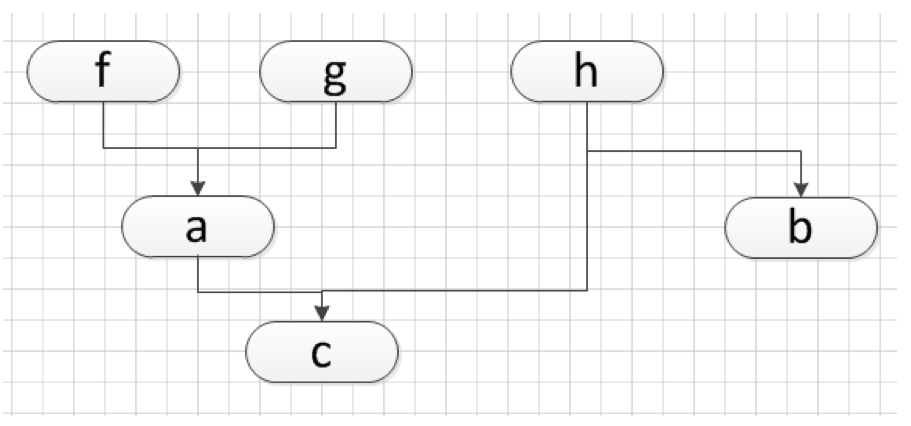
\includegraphics[scale=0.5]{flow.png}
\end{center}

We should only include formulae that belongs to functions that are
actually used. For example, to prove $a$'s contract, we should only
include $f$ and $g$ translations, and we would ask equinox:
$$ \dtrans{f},\dtrans{g},\dtrans{a},\strans{f},\strans{g} \vdash
\strans{a}$$


\section{Correctness of the translation}
For the translation to be useful, $\trans{M} \vdash \strans{f \in c} $
should imply that $f \in c$.


\section{Higher-orderness}
\label{ho}
Our current translation only considers fully applied functions and
first-order functions. For example, so far, we cannot give any
contract to $map$ because it would involve quantifying over a
function, a thing that is not first-order.

There is a possible workaround, which involves the ``app'' function
defined in our first-order logic. Assume we have a function $f$ that
is not fully applied somewhere in a module. We create the term
$f\_ptr$ which relates to $f$ by the equations given in \ref{ho-fig}

This way, we can emulate quantification over function by quantifying
on their $ptr$ counterpart.


\begin{figure*}
\label{ho-fig}
$$\etrans{e_1~e_2} = app(e_1,e_2)$$
$$ \forall x_1,\dots,x_n.~f(x_1,\dots,x_n) = app(app(\dots app(f\_ptr,x_1),x_2),\dots,x_n)$$
$$ \cf{f\_ptr} \tot \forall x_1,\dots,x_n.~\cf{x_1} \land \dots \land \cf{x_n} \to \cf{f(x_1,\dots,x_n)}$$
$$\forall f\_ptr,x.~\cf{f\_ptr} \land \cf{x} \to \cf{app(f\_ptr,x)}$$
\caption{Encoding of higher-orderness}
\end{figure*}

\section{Experiments}
That's how we roll.

\begin{figure*}
\label{comparison}
\begin{center}
    \begin{tabular}{l|c|c|c|c|c}
      Problem & Equinox & Equinox (+ weak) & SPASS & Vampire & E \\
      \hline
      Add.hs & 0.25 & 0.08 & 0.04 & 0.12 & 0.05\\
      BinaryTree.hs & 0.45 & 0.2 & 0.04 & 0.01 & 0.04 \\
      Branch.hs & 0.27 & 0.40 & 0.04 & 0.01 & 0.03 \\
      Copy.hs & 0.86 & 0.09 & 0.03 & 0.01 & 184.3 \\
      Head.hs & 0.32 & 0.29 & 0.03 & 0.03 & 4.2 \\
      Implies.hs & 3.24 & 0.32 & 0.06 & 0.02 & 0.11 \\
      Map.hs & 2.47 & 0.14 & 0.92 & 1.02 & $>$300 \\
      Mult.hs & $>$300 & 0.41 & 0.05 & 0.22 & 11.71 \\
      Multgt.hs & $>$300 & 1.24 & 0.62 & 1.31 & $>$300 \\
      NatEq.hs & 203.12 & 0.33 & 0.02 & 0.03 & 0.343 \\
      Odd.hs & 0.42 & 1.17 & 0.06 & 0.03 & $>$300 \\
      Reverse.hs & 72.32 & 0.12 & 0.05 & 0.02 & 0.038 \\
      Simple.hs & 0.07 & 0.04 & 0.01 & 0.01 & 0.022 \\
      Test.hs & 7.76 & 2.86 & 0.08 & 0.05 & $>$300 \\
      Test2.hs & 5.63 & 0.09 & 0.07 & 0.01 & 1.02 \\
    \end{tabular}
\end{center}
\caption{Comparison (in seconds) with other theorem provers}
\end{figure*}

\end{document}
